\documentclass[10pt]{beamer}
\usetheme[
%%% options passed to the outer theme
%    hidetitle,           % hide the (short) title in the sidebar
%    hideauthor,          % hide the (short) author in the sidebar
%    hideinstitute,       % hide the (short) institute in the bottom of the sidebar
%    shownavsym,          % show the navigation symbols
%    width=2cm,           % width of the sidebar (default is 2 cm)
%    hideothersubsections,% hide all subsections but the subsections in the current section
%    hideallsubsections,  % hide all subsections
%    left                % right of left position of sidebar (default is right)
  ]{Aalborg}
  
% If you want to change the colors of the various elements in the theme, edit and uncomment the following lines
% Change the bar and sidebar colors:
%\setbeamercolor{Aalborg}{fg=red!20,bg=red}
%\setbeamercolor{sidebar}{bg=red!20}
% Change the color of the structural elements:
%\setbeamercolor{structure}{fg=red}
% Change the frame title text color:
%\setbeamercolor{frametitle}{fg=blue}
% Change the normal text color background:
%\setbeamercolor{normal text}{bg=gray!10}
% ... and you can of course change a lot more - see the beamer user manual.

\usepackage[utf8]{inputenc}
%\usepackage[english]{babel}
\usepackage[spanish]{babel}
\usepackage[T1]{fontenc}
\usepackage[demo]{graphicx}   
% Or whatever. Note that the encoding and the font should match. If T1
% does not look nice, try deleting the line with the fontenc.

\usepackage[table,xcdraw]{xcolor}
\usepackage{helvet}
\usepackage{tikz}
\usetikzlibrary{shapes,arrows,positioning}

%\usepackage{minted}
\usepackage{animate}
\usepackage{media9}
\usepackage[makeroom]{cancel}


\usepackage{listings}
\usepackage{color}
\definecolor{codegreen}{rgb}{0,0.6,0}
\definecolor{codegray}{rgb}{0.5,0.5,0.5}
\definecolor{codepurple}{rgb}{0.58,0,0.82}
\definecolor{backcolour}{rgb}{0.95,0.95,0.92}
 
\lstdefinestyle{mystyle}{
    backgroundcolor=\color{backcolour},   
    commentstyle=\color{codegreen},
    keywordstyle=\color{magenta},
    numberstyle=\tiny\color{codegray},
    stringstyle=\color{codepurple},
    basicstyle=\footnotesize,
    breakatwhitespace=false,         
    breaklines=true,                 
    captionpos=b,                    
    keepspaces=true,                 
    numbers=left,                    
    numbersep=5pt,                  
    showspaces=false,                
    showstringspaces=false,
    showtabs=false,                  
    tabsize=2
}
 
\lstset{style=mystyle}


% colored hyperlinks
\newcommand{\chref}[2]{%
  \href{#1}{{\usebeamercolor[bg]{Aalborg}#2}}%
}

\title[Análisis y Diseño de Circuitos Eléctricos]% optional, use only with long paper titles
{Análisis y Diseño de Circuitos Eléctricos}

\subtitle{Conceptos de Electromagnetismo}  % could also be a conference name

\date{\today}

\author[Víctor Medrano Zarazúa] % optional, use only with lots of authors
{
  Víctor Medrano Zarazúa\\
  \href{mailto:victor_medrano@my.uvm.edu.mx}{{\tt victor\_medrano@my.uvm.edu.mx}}
}
% - Give the names in the same order as they appear in the paper.
% - Use the \inst{?} command only if the authors have different
%   affiliation. See the beamer manual for an example

\institute[
%  {\includegraphics[scale=0.2]{aau_segl}}\\ %insert a company, department or university logo
  %Dept.\ of Electronic Systems\\
  Universidad del Valle de México\\
  Campus Monterrey
] % optional - is placed in the bottom of the sidebar on every slide
{% is placed on the bottom of the title page
  %Department of Electronic Systems\\
  Universidad del Valle de México\\
  Campus Monterrey
  %Universidad Autónoma de Nuevo León\\
  %Facultad de Ingeniería Mecánica y Eléctrica
  
  %there must be an empty line above this line - otherwise some unwanted space is added between the university and the country (I do not know why;( )
}

% specify the logo in the top right/left of the slide
\pgfdeclareimage[height=1cm]{mainlogo}{AAUgraphics/UVM} % placed in the upper left/right corner
\logo{\pgfuseimage{mainlogo}}

% specify a logo on the titlepage (you can specify additional logos an include them in 
% institute command below
\pgfdeclareimage[height=1.5cm]{titlepagelogo}{AAUgraphics/UVM} % placed on the title page
%\pgfdeclareimage[height=1.5cm]{titlepagelogo2}{AAUgraphics/aau_logo_new} % placed on the title page
\titlegraphic{% is placed on the bottom of the title page
  \pgfuseimage{titlepagelogo}
%  \hspace{1cm}\pgfuseimage{titlepagelogo2}
}

%\definecolor{UniBlue}{RGB}{255,255,255}

\tikzset{
block/.style={
  draw, 
  fill=blue!20, 
  rectangle, 
  minimum height=3em, 
  minimum width=6em
  },
 gain/.style={
    draw,
    fill=blue!20, 
    isosceles triangle,
    minimum height = 3em,
    isosceles triangle apex angle=60
    },
sum/.style={
  draw, 
  fill=blue!20, 
  circle, 
  },
input/.style={coordinate},
output/.style={coordinate},
pinstyle/.style={
  pin edge={to-,thin,black}
  }
}  

\begin{document}
% the titlepage


%\setbeamercolor{title}{fg=UniBlue}
%\setbeamercolor{normal text}{fg=UniBlue}
%\setbeamercolor{Aalborg}{fg=black,bg=black}


{\aauwavesbg
\begin{frame}[plain,noframenumbering] % the plain option removes the sidebar and header from the title page
  \titlepage
\end{frame}}
%%%%%%%%%%%%%%%%

% TOC
\begin{frame}{Contenido}{}
\tableofcontents
\end{frame}
%%%%%%%%%%%%%%%%
\section{Introducción}
\begin{frame}{Introducción}{}
\begin{block}{Repasemos conceptos...}
\begin{itemize}
Es importante que repasemos conceptos de \textcolor{blue}{electromagnetismo} y posteriormente dar paso a nuevos conceptos para comprender el análisis y diseño de circuitos.
\end{itemize}
\end{block}
\vspace{-0.1in}
\begin{figure}[h!]
\centering

\includegraphics [scale=0.32]{spongeschool}
%\caption{Bobina Tesla}
\label{fig:tesla}
\end{figure}

\end{frame}

%\begin{frame}{Introducción}{}
%\begin{block}{Tenemos tecnología...}
%\begin{itemize}
%Hoy vivimos en un mundo predominantemente eléctrico. Las dos áreas primarias de la electrotecnología que permean esencialmente todos los aspectos de nuestras vidas son la potencia y la información.
%\end{itemize}
%\end{block}

%\begin{figure}[h!]
%\centering
%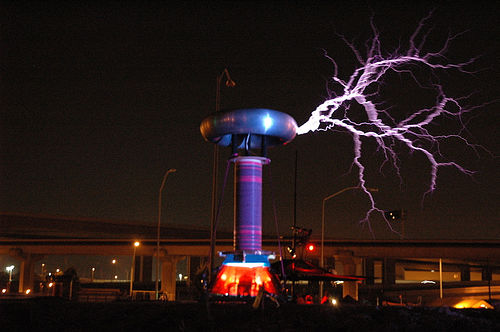
\includegraphics [scale=0.32]{teslacoil}
%\caption{Bobina Tesla}
%\label{fig:tesla}
%\end{figure}
%\end{frame}


\section{Carga eléctrica}
\begin{frame}{Carga eléctrica}{}

\begin{block}{Carga}
Es una propiedad eléctrica de las partículas eléctricas de las que se compone la materia, medida en Coulombs (C).
\end{block}

\begin{figure}[h!]
\centering
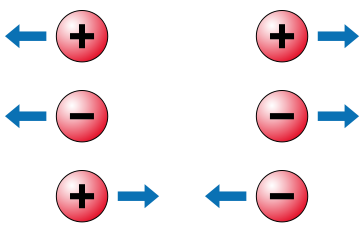
\includegraphics [scale=0.32]{charges}
%\caption{Bobina Tesla}
\label{fig:cargas}
\end{figure}

\end{frame}

\section{Conductores, aislantes y semiconductores}
\begin{frame}{Conductores, aislantes y semiconductores}{Back to chemistry...}

\begin{itemize}
    \item Los conductores están formados por átomos cuyos electrones exteriores, o de valencia, están débilmente ligados a sus núcleos.
    \item Los electrones de valencia son aquellos que se encuentran en la capa más externa del átomo. Tienen la particularidad de requerir menos energía para separarse del átomo padre. 
    \item Uno de los materiales que más utilizamos para mover carga es el cobre.
\end{itemize}
\medskip
\begin{columns}[c]
\column{1.3in}
\framebox{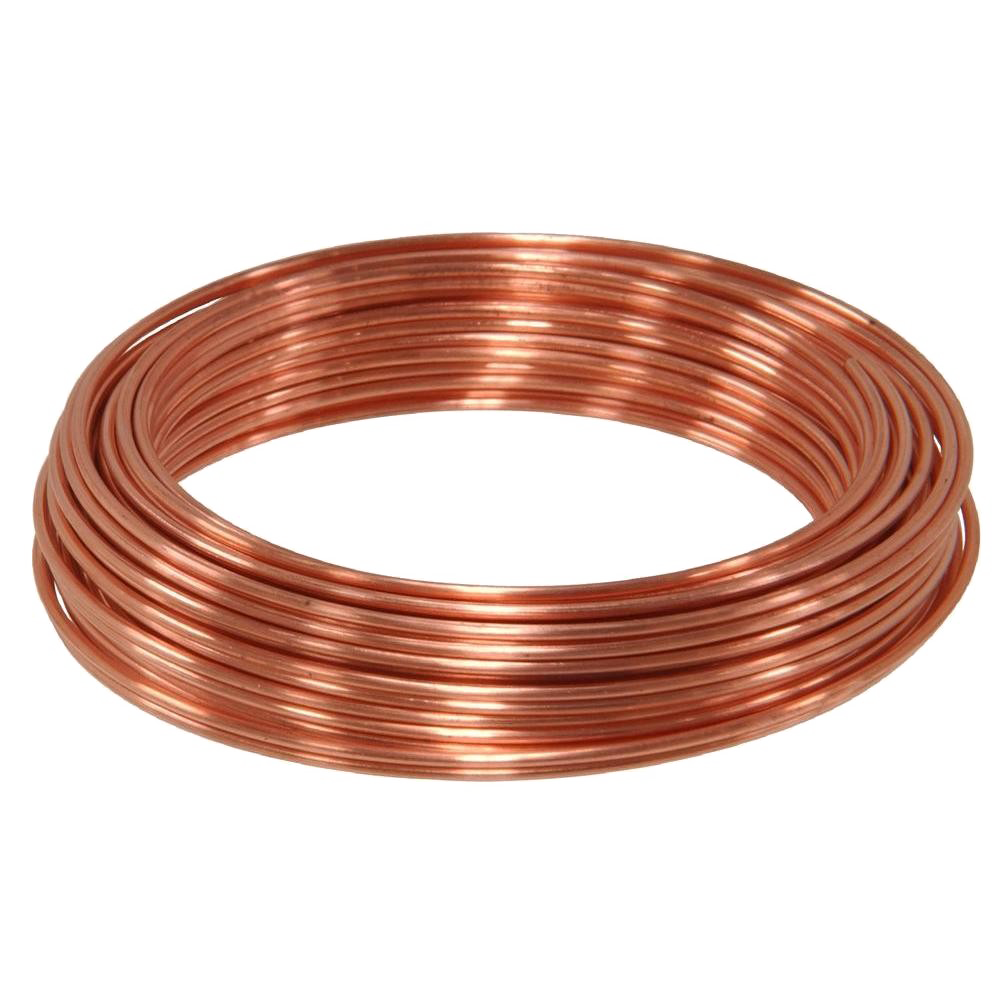
\includegraphics[width=1.3in]{copperwire}}
\column{1.3in}
\framebox{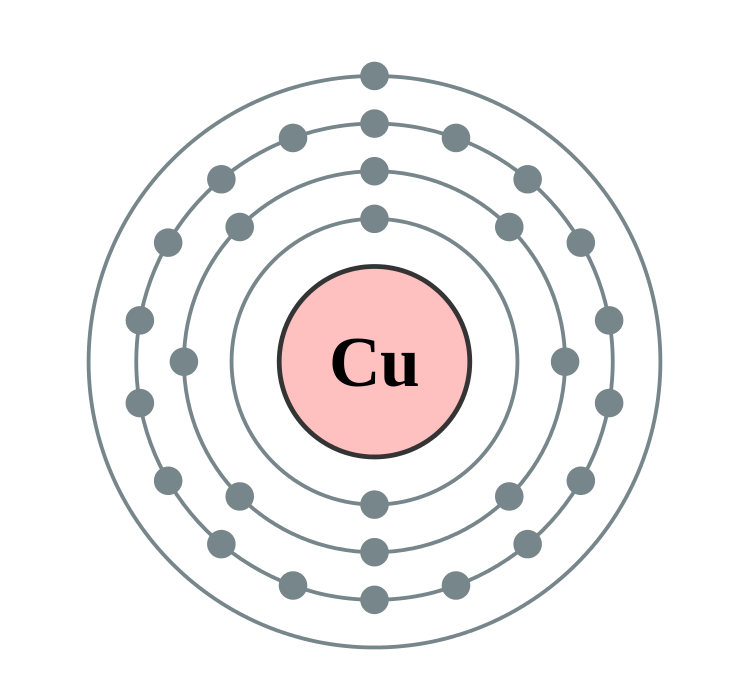
\includegraphics[width=1.3in]{cuatom}}
\end{columns}
%\end{block}

\end{frame}

\begin{frame}{Conductores, aislantes y semiconductores}{Back to chemistry...}

\begin{itemize}
    \item Los aislantes son materiales cuyos electrones exteriores están fuertemente ligados a sus núcleos. Las fuerzas eléctricas moderadas no son capaces de arrancarlos de sus átomos.
\end{itemize}
\medskip
\begin{figure}[h!]
\centering
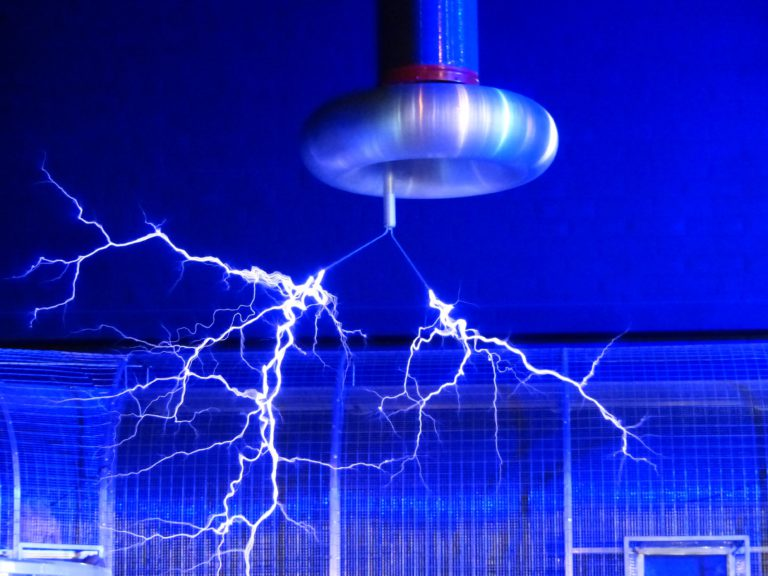
\includegraphics [scale=0.25]{voltaicarc}
\label{fig:first}
\end{figure}
\end{frame}


\begin{frame}{Conductores, aislantes y semiconductores}{Back to chemistry...}

\begin{itemize}
    \item Los materiales semiconductores están entre los aislantes y los conductores. Usualmente actúan como aislantes, pero bajo ciertas circunstancias podemos hacer que se comporten como conductores.
\end{itemize}
\medskip
\medskip
\begin{columns}[c]
\column{1.5in}
\framebox{
\includegraphics[width=1.5in]{greensemi.png}}
\column{1.5in}
\framebox{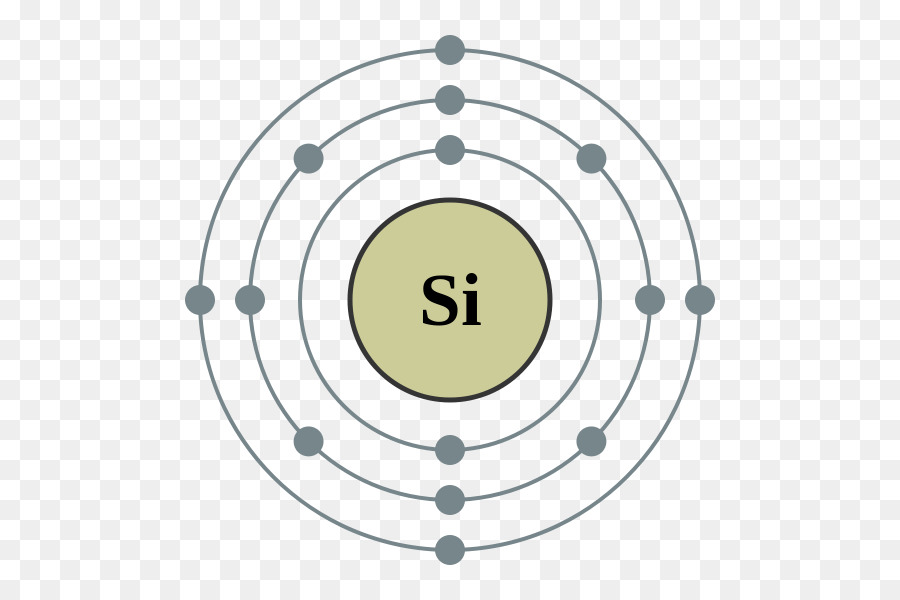
\includegraphics[width=1.5in]{siatom.jpg}}
\end{columns}
\end{frame}

\section{Corriente eléctrica}
\begin{frame}{Corriente Eléctrica}{}

\begin{block}{Corriente Eléctrica}
Es la velocidad de cambio de la carga respecto al tiempo, medida en amperes (A). En otras palabras, es el flujo de carga.
\end{block}
\medskip
\begin{figure}[h!]
\centering
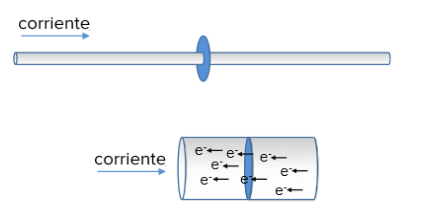
\includegraphics [scale=0.45]{current}
\label{fig:first}
\end{figure}
\end{frame}

\begin{frame}{Corriente Eléctrica}{}
Ya que la corriente es la cantidad de carga que pasa a través de una frontera en una cantidad de tiempo, podemos expresarla matemáticamente con la ecuación:
\begin{equation}
    i = \frac{dq}{dt}
\end{equation}
\end{frame}

\begin{frame}{Sentido de la corriente}{}
\begin{block}{¿Qué es lo que transporta la corriente en un metal?}
En los metales, los electrones pueden moverse libremente; al hacerlo, generan la corriente dentro de estos materiales. Aunque los electrones tienen carga negativa y hacen casi todo el trabajo en la mayoría de los circuitos eléctricos, definimos una corriente positiva como la dirección en la que se movería una carga positiva. Esta es una muy vieja convención histórica.
\end{block}

\begin{figure}[h!]
\centering
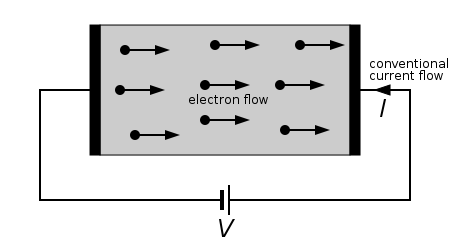
\includegraphics [scale=0.45]{electronflow}
\label{fig:first}
\end{figure}
\end{frame}


\begin{frame}{Sentido de la corriente}{}
\begin{block}{¿Las cargas positivas pueden transportar corriente?}
 Sí. En el agua salada, tanto las cargas positivas como las negativas transportan corriente. 
\end{block}

\begin{figure}[h!]
\centering
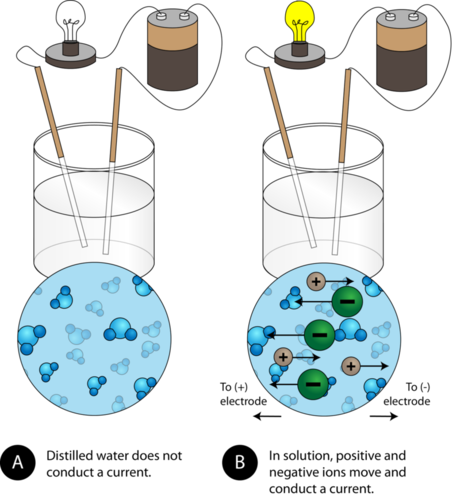
\includegraphics [scale=1.3]{saltwater}
\label{fig:first}
\end{figure}
\end{frame}

\begin{frame}{Sentido de la corriente}{}
\begin{block}{¿Cuál es la velocidad de la corriente?}
Usualmente, la corriente no trata de metros por segundo, sino de carga por segundo. Es más común que respondamos la pregunta "¿cuánta corriente fluye?".
\end{block}

\begin{block}{¿Cómo sí hablamos de la corriente?}
Cuando discutimos sobre la corriente, términos como \textbf{a través} y \textbf{en} tienen mucho sentido. La corriente fluye \textbf{a través} de un resistor; la corriente fluye \textbf{en} un alambre.
\end{block}

\end{frame}

\section{Voltaje}

\begin{frame}{Voltaje}{}
\begin{block}{El voltaje se parece a la gravedad}
\begin{itemize}
    \item Para una masa $m$, un cambio en la altura $h$ corresponde a un cambio en la energía potencial, $\Delta U = mg\Delta h$.
    \item Para una partícula cargada $q$, un voltaje $V$ corresponde a un cambio en la energía potencial, $\Delta U = qV$.
\end{itemize}
\end{block}

\begin{figure}[h!]
\centering
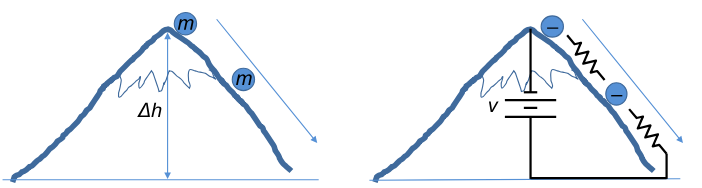
\includegraphics [scale=0.39]{mountvolt}
\label{fig:first}
\end{figure}

\end{frame}

\begin{frame}{Voltaje}{}
Podemos expresar matemáticamente el voltaje entre dos puntos como el cambio en energía que experimenta una carga:

\begin{equation}
    V = \frac{dU}{dq}
\end{equation}
\end{frame}

\section{Potencia}

\begin{frame}{Potencia}{}
\begin{block}{}
La potencia está definida como la tasa a la que la energía ($U$) se transforma o se transfiere en el tiempo. Medimos la potencia en unidades de joules/segundo, también conocidas como watts.

\begin{equation}
    P = \frac{dU}{dt}
\end{equation}
\end{block}

\end{frame}

\begin{frame}{Potencia}{}
Un circuito eléctrico es capaz de transferir potencia. La corriente es la razón de flujo de carga, y el voltaje mide la energía por unidad de carga que se transfiere. Podemos insertar estas definiciones en la ecuación para la potencia:

\begin{equation}
    P = \frac{dU}{dt} = \frac{dU}{\cancel{dq}} \frac{\cancel{dq}}{dt} = V i
\end{equation}
\end{frame}

\section{En resumen...}
\begin{frame}{En resumen...}{}
Estos modelos mentales para la corriente y el voltaje nos permitirán empezar a estudiar toda clase de circuitos eléctricos interesantes.
\end{frame}

%%%%%%%%%%%%%%%%%%%%%%%%%%%%5
\section{Información de contacto}
% contact information
\begin{frame}{Feedback}{Información de contacto}
En caso de comentarios, sugerencias, preguntas o errores en las diapositivas no dudes en contactarme.
  \begin{center}
    \insertauthor\\
    \chref{https://mixlaab.github.io}{https://mixlaab.github.io}\\
    WA: 8119022700\\
    %9220 Aalborg Ø
  \end{center}
\end{frame}
%%%%%%%%%%%%%%%%

{\aauwavesbg%
\begin{frame}[plain,noframenumbering]%
  \finalpage{Fin}
\end{frame}}
%%%%%%%%%%%%%%%%

\end{document}
